\section{Strategies and harness formats}
\label{sec:row-1}

The experiment shows that a model can use a long input unevenly, so we turn to the harnesses lane of the map, how a harness chooses what each call receives: the ways to manage context, one measured method of extraction, the abstractive rewriting that harnesses use, the methods learned for agents since 2025, the compaction strategies one by one, the formats of Pi, Claude Code and Codex, and the tools LangGraph supplies.

\subsection{Context: retain, retrieve, extract, rewrite}
\label{sec:it-7-1}

\bi
\item \textbf{Retain} keeps selected original messages or results.
\item \textbf{Retrieve} fetches material by query or reference when needed.
\item \textbf{Extract} keeps only the informative tokens of what stays.
\item \textbf{Rewrite} replaces a span with a generated summary.
\ei

These four ways are the course's organizing scheme for Part II. Retain keeps original messages or results as they were written. Retrieve fetches material by query or by reference when it is needed. Extract keeps only the informative tokens of what stays. Rewrite replaces a span with a generated summary. Retrieval draws on a large literature, such as retrieval-augmented generation (Lewis et al., Retrieval-Augmented Generation for Knowledge-Intensive NLP Tasks, NeurIPS 2020), which stays supporting reading. The four ways also sort the harnesses lane of the map: RAG retrieves, LLMLingua and LLMLingua-2 extract, MemGPT retrieves and rewrites, SWE-agent retains its latest observations whole, and ACON rewrites. The next slides open extraction and rewriting, then compare the compaction strategies one by one.

The ledger line and its four forms are illustrative. The extract row drops only the colon and the two commas, shown in grey, a small instance of the keep-or-drop choice that LLMLingua-2's classifier makes for every word. The rewrite row says the same facts in fewer, new words. The four-way split is the course's scheme, attributed to no paper.

\begin{figure}[htbp]
\centering
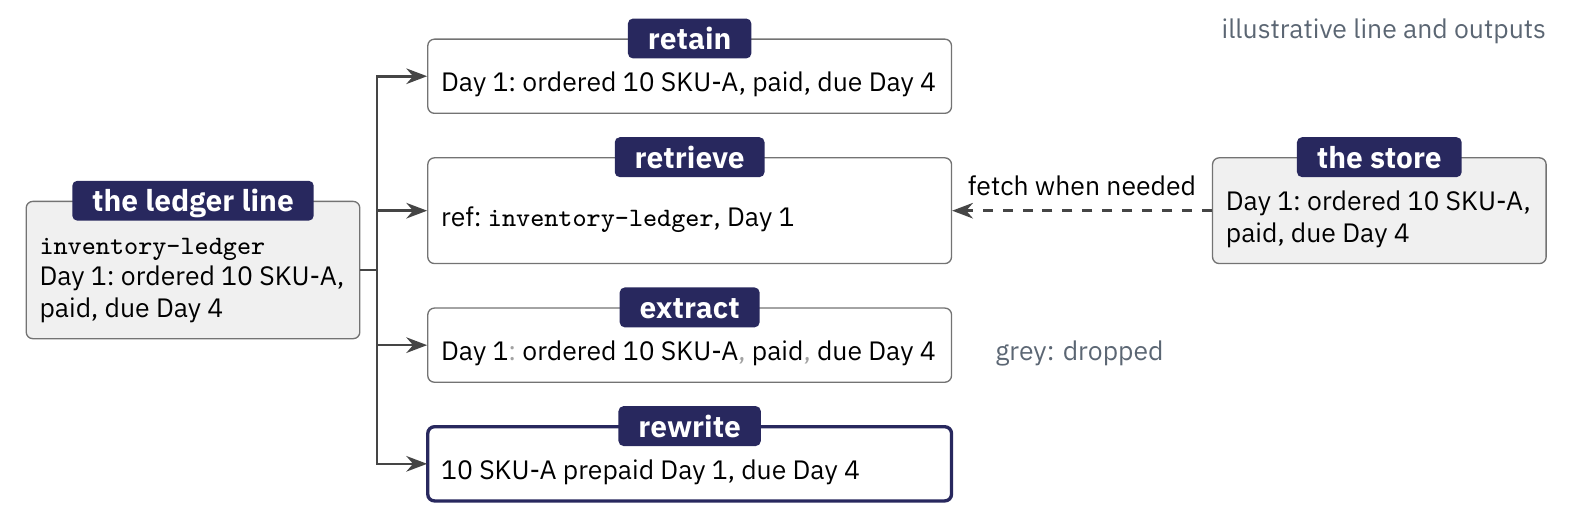
\includegraphics[width=\linewidth]{context/four-ways-4.png}
\caption{Context: retain, retrieve, extract, rewrite The figure as it stands after the build's last click.}
\label{fig:four-ways-4}
\end{figure}

\paragraph{The figure, stage by stage.}
\be
\item Retain: the later call receives the ledger line from inventory-ledger word for word, Day 1: ordered 10 SKU-A, paid, due Day 4. The order, the payment and the due date all reach the call.
\item Retrieve: the context carries only the reference ref: inventory-ledger, Day 1, and the line itself stays in the store. The dashed arrow, fetch when needed, brings the line back when a later call asks for it.
\item Extract: the row keeps every word of the ledger line in its order. The colon and the two commas are dropped, and the key grey: dropped marks them.
\item Rewrite: the new sentence 10 SKU-A prepaid Day 1, due Day 4 keeps every fact in fewer words, so its box is shorter than the line's. The word prepaid never appears in the ledger line, which shows that the sentence is generated.
\ee

\begin{takeaway}A context policy determines what to keep, fetch, shorten or rewrite.\end{takeaway}

\subsection{Extractive compression selects tokens}
\label{sec:it-7-2}

\bi
\item \textbf{LLMLingua-2} (Pan et al., 2024) trains a classifier to keep or drop each token.
\item \textbf{The method:} trained on GPT-4's compressions, it reads both sides of a token.
\item \textbf{The evaluation:} task scores, compression and latency on several datasets.
\ei

Zhuoshi Pan et al., LLMLingua-2: Data Distillation for Efficient and Faithful Task-Agnostic Prompt Compression, Findings of ACL 2024, 963--981 (doi:10.18653/v1/2024.findings-acl.57). This is the navy work of the map's harnesses lane, the mechanism Part II studies in depth. Its origin is LLMLingua (Jiang et al., LLMLingua: Compressing Prompts for Accelerated Inference of Large Language Models, EMNLP 2023), and LongLLMLingua (Jiang et al., LongLLMLingua: Accelerating and Enhancing LLMs in Long Context Scenarios via Prompt Compression, ACL 2024) is its long-context extension.

LLMLingua-2 trains a token classifier on an extractive compression dataset distilled from GPT-4. GPT-4 compresses MeetingBank transcripts, in chunks of at most 512 tokens, by deleting words, and an alignment algorithm turns each compression into a keep or drop label for every original word (section 3.2). The classifier uses the context on both sides of each token to decide whether to keep it. The evaluations compare compression with task scores and latency on MeetingBank and on out-of-domain datasets. The reported gains apply to those test conditions, so we promise no fixed compression ratio or speed-up.

The limit, which the slide \hyperref[sec:it-7-4b]{``Extractive selection keeps key tokens.''} shows, is that deleting tokens can lose the meaning the task needs, so we test every use on the task. Inside agents the loss is measured: the slide \hyperref[sec:it-7-3b]{``Agents now learn what their context keeps.''} follows the work since 2025 that compacts an agent's history instead of its words.

The line ``ordered 10 SKU-A, paid, due Day 4 unless cancelled'' extends the deck's running ledger line for this slide, and its keep and drop labels are the course's example. LLMLingua-2's classifier did not produce them. The paper distills its training data from GPT-4.

\begin{figure}[htbp]
\centering
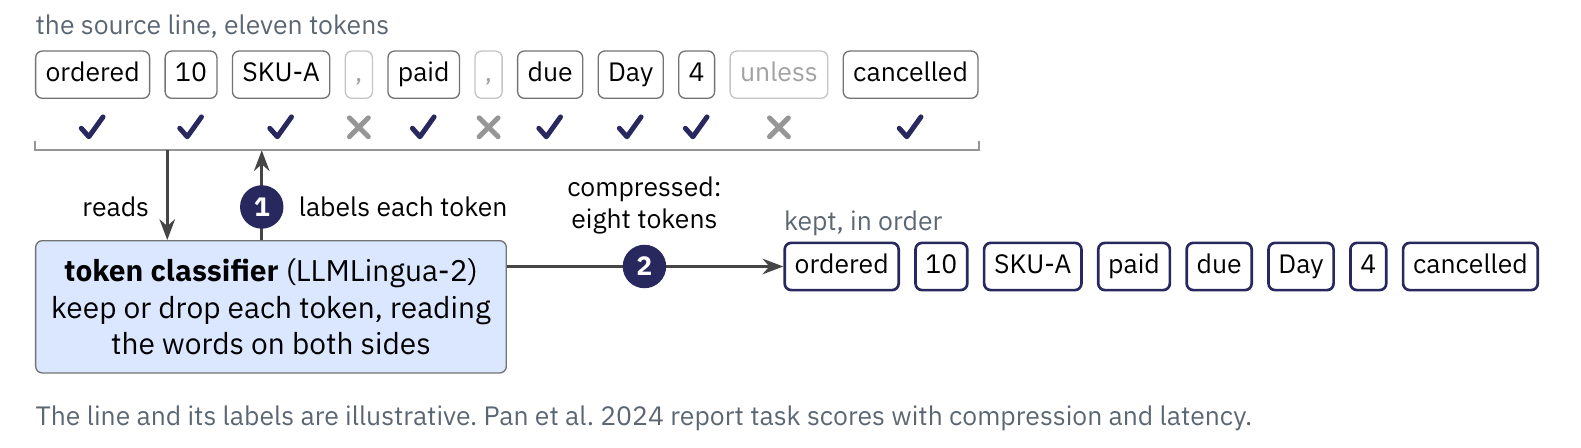
\includegraphics[width=\linewidth]{context/extractive-3.png}
\caption{Extractive compression selects tokens. The figure as it stands after the build's last click.}
\label{fig:extractive-3}
\end{figure}

\paragraph{The figure, stage by stage.}
\be
\item The source line, eleven tokens: ordered, 10, SKU-A, a comma, paid, a comma, due, Day, 4, unless and cancelled. As written, the order stands unless someone cancels it, and the dashed box marks where the token classifier will stand.
\item The token classifier (LLMLingua-2) reads the line, and arrow 1, 'labels each token', marks every token keep or drop, reading the words on both sides. Eight tokens get a navy tick, and the two commas and unless get a grey cross.
\item Arrow 2, 'compressed: eight tokens', leads to the row 'kept, in order': ordered, 10, SKU-A, paid, due, Day, 4 and cancelled. The two commas and unless fade in the source line because the next call never receives them.
\ee

\begin{takeaway}A compressed input is judged by the task it must support.\end{takeaway}

\subsection{Abstractive compaction rewrites history}
\label{sec:it-7-3}

\bi
\item \textbf{Input:} selected conversation history or observations.
\item \textbf{Transformation:} a model summarizes what the next step needs.
\item \textbf{Replacement:} later calls carry the summary plus retained material.
\item \textbf{Risk:} omissions and unsupported claims change what the next call believes.
\ei

Abstractive compaction takes selected history or observations, has a model write a shorter summary of the information the next step needs, and assembles later requests from that summary plus any material kept on purpose. An omission or an unsupported statement in the summary changes what the next call believes.

The article of Anthropic's Applied AI team (Effective context engineering for AI agents, September 29, 2025) describes compaction as a summary that replaces the history in a fresh context. Its compaction section warns that overly aggressive compaction can lose context whose importance appears only later, and it recommends tuning the summary prompt on complex agent traces. This is engineering guidance rather than a controlled comparison. The course groups the methods as retain, retrieve, extract and rewrite, and the long-horizon example uses abstractive compaction.

The five messages stand for a longer history, and the token counts are illustrative. The next request's three parts (the system prompt, the summary, the recent messages) follow Pi's documented rebuild. No stage shows an unsupported statement, and the faithfulness check of the evaluation section returns to that half of the risk.

\begin{figure}[htbp]
\centering
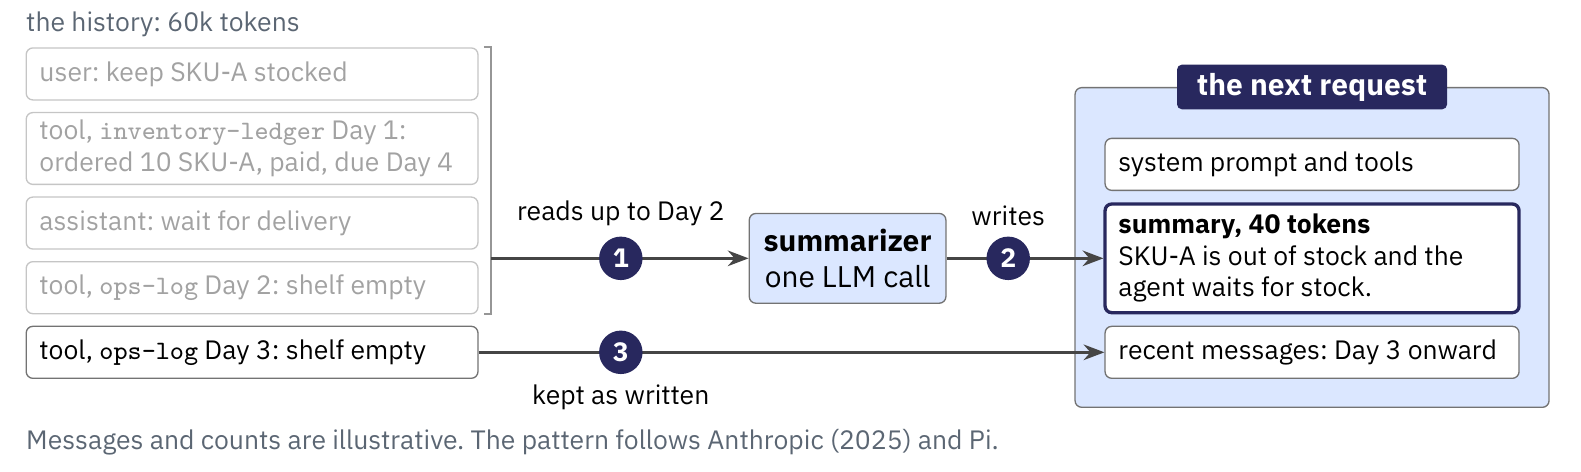
\includegraphics[width=\linewidth]{context/abstractive-3.png}
\caption{Abstractive compaction rewrites history. The figure as it stands after the build's last click.}
\label{fig:abstractive-3}
\end{figure}

\paragraph{The figure, stage by stage.}
\be
\item The history: 60k tokens in five messages, from 'user: keep SKU-A stocked' and 'tool, inventory-ledger Day 1: ordered 10 SKU-A, paid, due Day 4' to the two ops-log lines 'shelf empty' on Days 2 and 3. The dashed box marks where the summarizer will stand.
\item The summarizer, one LLM call, reads up to Day 2 and writes 'summary, 40 tokens: SKU-A is out of stock and the agent waits for stock.' The four messages it read fade because the next call will not receive them, and the Day 3 log stays dark.
\item The next request holds 'system prompt and tools', the summary and 'recent messages: Day 3 onward'. Arrow 3 carries the Day 3 log into it, kept as written.
\ee

\begin{takeaway}A generated summary becomes another representation that needs checking.\end{takeaway}

\subsection{Agents now learn what their context keeps}
\label{sec:it-7-3b}

\bi
\item \textbf{Token pruning:} deleting words inside an agent's messages cost 17 points.
\item \textbf{Masking:} a rule replaces old tool observations with placeholders.
\item \textbf{Learned guidelines:} a compressor follows instructions refined on failed runs.
\item \textbf{Trained folding:} the agent learns by RL to fold each finished subtask.
\ei

LLMLingua-2 compresses one prompt for any task. Since 2025, compaction research has turned to agents, whose histories grow with every tool call, and it has moved the decision about what to drop from a fixed rule to a tuned compressor and then to the agent's own trained policy. Each row of the figure is one step, with a result that its paper compares against the same model with the full history.

Token pruning inside an agent: ACON (Minki Kang and colleagues, ACON: Optimizing Context Compression for Long-horizon LLM Agents, ICML 2026, arXiv:2510.00615) includes an LLMLingua baseline. On AppWorld with gpt-4.1, accuracy falls from 56.0\% with the full history to 39.3\%. SWE-Pruner (Wang and colleagues, a 2026 preprint) reports the same direction on 50 tasks of SWE-bench Verified: LLMLingua-2 takes success from 62\% to 54\%.

Masking: The Complexity Trap (Tobias Lindenbauer and colleagues, DL4C workshop at NeurIPS 2025, arXiv:2508.21433) replaces every tool observation older than the last ten turns with a placeholder and keeps all reasoning and actions. With Qwen3-Coder 480B in SWE-agent on SWE-bench Verified, masking solves 54.8\% of the tasks at \$0.61 each, an LLM summary 53.8\% at \$0.64, and the raw history 53.4\% at \$1.29. Observations make up about 84\% of a turn's tokens, which is why masking saves so much. It is the agent's version of keeping the recent turns, and LangGraph's ClearToolUsesEdit and Anthropic's context editing implement it.

Learned guidelines: ACON compresses the history, or one long observation, with an LLM that follows written guidelines. An optimizer LLM refines the guidelines from runs that succeed without compression and fail with it, and the compressor is then distilled into a small model. On AppWorld with gpt-4.1, accuracy is 56.5\% against 56.0\% without compression, while the peak context falls from 9.93K to 7.33K tokens. Across its benchmarks, peak tokens fall by 26 to 54\%.

Trained folding: Context-Folding (Weiwei Sun and colleagues, Scaling Long-Horizon Agent via Context Folding, ICML 2026, arXiv:2510.11967) trains the agent with reinforcement learning (FoldGRPO) to branch into a subtask and fold it into one summary when the subtask ends. Seed-OSS-36B with a 32K active context reaches 58.0\% on SWE-bench Verified and 62.0\% on BrowseComp-Plus, against 57.4\% and 54.0\% for an RL-trained ReAct agent with a 327K window. MEM1 (Zhou and colleagues, ICLR 2026) and AgentFold (Ye and colleagues, ICLR 2026) train similar policies.

The vendors have built the last step into their models and APIs. OpenAI describes GPT-5.1-Codex-Max (November 19, 2025) as natively trained to work across context windows through compaction, its Responses API compacts on request or on the server, and the Claude API has compacted on the server since February 5, 2026.

The six turns, the block widths and the turns each method changes are illustrative: the paper's masking keeps the last ten turns where the figure keeps two. Each row's numbers come from its own benchmark and models, as the note under the figure says, so they compare only within a row. ACON's LLMLingua baseline does not name its checkpoint.

\begin{figure}[htbp]
\centering
\includegraphics[width=\linewidth]{context/agent-compaction-5.png}
\caption{Agents now learn what their context keeps. The figure as it stands after the build's last click.}
\label{fig:agent-compaction-5}
\end{figure}

\paragraph{The figure, stage by stage.}
\be
\item The history: six turns of an agent, each a short action in blue and a wide tool observation in grey. Observations are about 84\% of a turn's tokens, the share The Complexity Trap measured in SWE-agent. The grey note says that each row's numbers come from its own benchmark.
\item Token pruning: words are deleted inside every message, as LLMLingua does. Inside an agent, ACON's LLMLingua baseline falls from 56.0\% with the full history to 39.3\% on AppWorld.
\item Masking: a rule replaces the old observations with short placeholders and keeps every action. On SWE-bench Verified, masking solves 54.8\%, 52\% cheaper than the raw history.
\item Learned guidelines: a compressor rewrites the old turns into one summary, following guidelines learned from failed runs. ACON keeps AppWorld at 56.5\% while the peak context falls 26\%.
\item Trained folding: the agent itself, trained by reinforcement learning, folds a finished subtask into one summary. Context-Folding reaches 58.0\% on SWE-bench Verified with 32K of context, against 57.4\% with 327K.
\ee

\begin{takeaway}Newer compaction is measured, and often trained, on the agent's own tasks.\end{takeaway}

\subsection{Recency keeps the last turns}
\label{sec:it-7-4a}

\bi
\item \textbf{How:} the harness keeps the most recent turns and drops older ones.
\item \textbf{Strength:} no extra call and no extra tokens.
\item \textbf{Failure:} an old but open commitment is dropped.
\ei

Recency keeps the most recent turns and drops the older ones, so it costs nothing beyond the drop. Its failure is an old commitment that is still open: the order paid on Day 1 leaves the context while its delivery is still due. Recency is the fallback when nothing else is in place, and Pi keeps the most recent messages beside its summary (the slide \hyperref[sec:it-7-5a]{``Pi compacts into a structured summary.''}).

Agent harnesses apply the same idea to tool results. SWE-agent (Yang et al., NeurIPS 2024) keeps the last five observations whole and collapses each older one to a single line. The Complexity Trap (Lindenbauer et al., NeurIPS 2025 workshop) compared the same masking, keeping the observations of the last ten turns, against LLM summarization on SWE-bench Verified: masking halved the cost of the unmanaged agent and matched the solve rate of summarization. Masking collapses old tool output and keeps every thought and action, so a commitment the agent wrote down stays in the context (SWE-agent keeps the agent's plan and actions, Yang et al., section 3). The figure's recency drops whole turns, actions included. A solve rate on SWE-bench Verified does not show whether an old open commitment survived.

The eight turns and the context of the last five are illustrative. Pi sizes its kept messages in tokens (keepRecentTokens, 20k tokens by default) where the figure counts turns, and ``the cheapest strategy'' is the course's comparison rather than a measurement.

\begin{figure}[htbp]
\centering
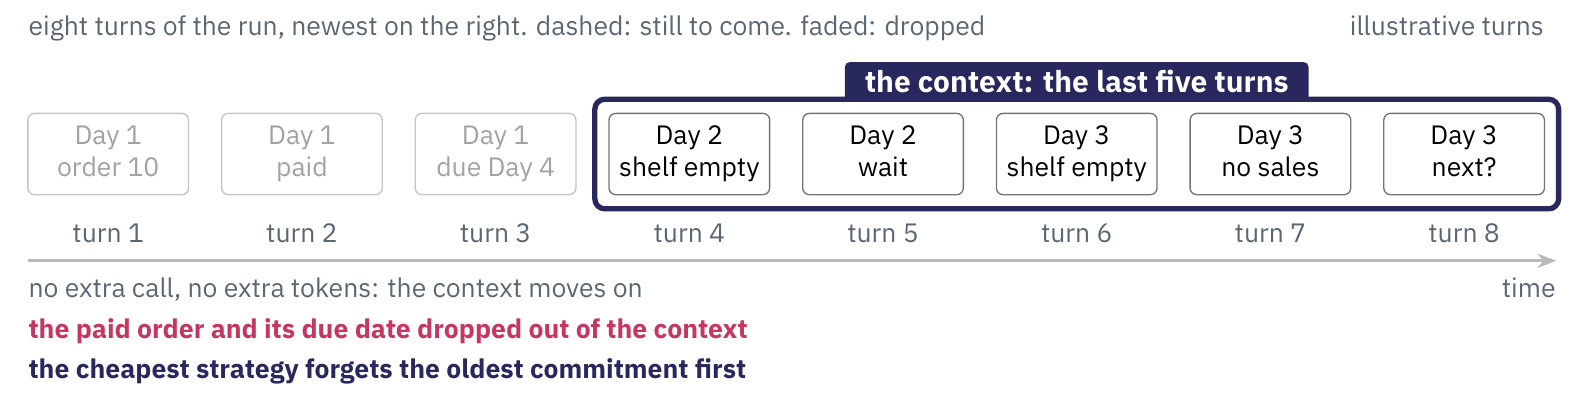
\includegraphics[width=\linewidth]{context/recency-3.png}
\caption{Recency keeps the last turns. The figure as it stands after the build's last click.}
\label{fig:recency-3}
\end{figure}

\paragraph{The figure, stage by stage.}
\be
\item The context: the last five turns holds turns 1 to 5, and turns 1 to 3 carry order 10, paid and due Day 4 from Day 1. The dashed turns 6 to 8 are still to come.
\item The context moves on to turns 3 to 7, and turns 1 and 2, order 10 and paid, fade as dropped. The note gives the cost: no extra call, no extra tokens: the context moves on.
\item The context moves again to turns 4 to 8, and turn 3, due Day 4, fades. The magenta line names the loss, the paid order and its due date dropped out of the context, and the navy line gives the verdict, the cheapest strategy forgets the oldest commitment first.
\ee

\begin{takeaway}Recency adds no cost, and an open commitment leaves with its old turns.\end{takeaway}

\subsection{Extractive selection keeps key tokens}
\label{sec:it-7-4b}

\bi
\item \textbf{How:} a classifier keeps the informative tokens and drops the rest.
\item \textbf{Strength:} cheap and model-agnostic.
\item \textbf{Failure:} one dropped word can flip the meaning.
\ei

Extractive selection keeps the informative tokens and drops the rest, so it is cheap and works with any downstream model. The kept tokens read as a terse excerpt of the source. One dropped word can flip the meaning, which is why the compressed input is tested on the task. LLMLingua-2 (the slide \hyperref[sec:it-7-2]{``Extractive compression selects tokens.''}) is the worked method.

The dropped ``unless'' is the course's example. The strength follows from the method: a small classifier runs once over the input, and any model can read the kept tokens.

\begin{figure}[htbp]
\centering
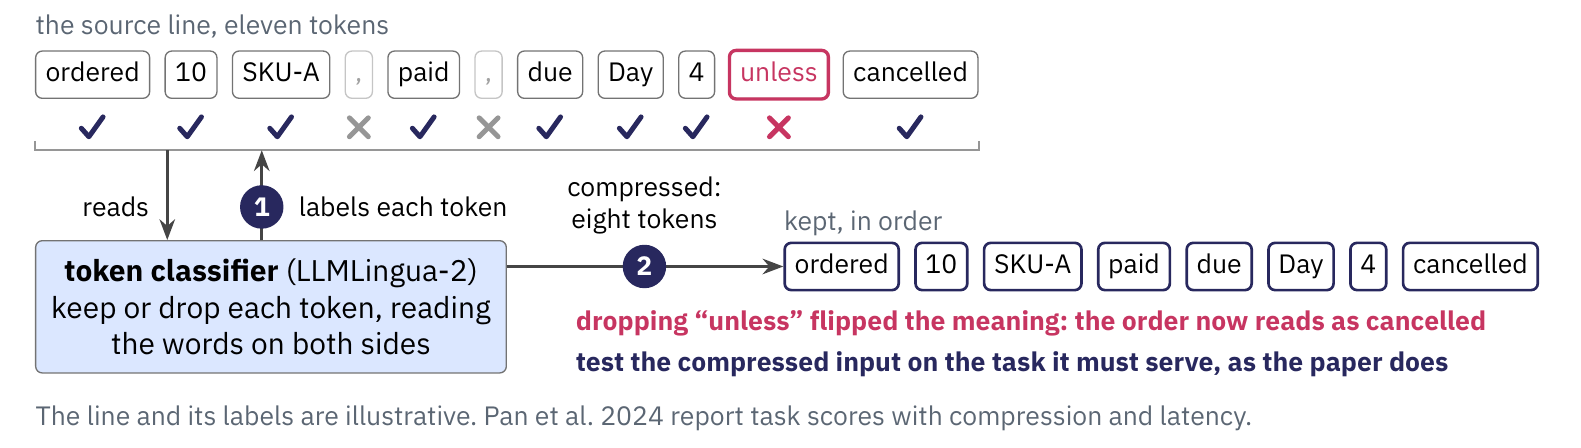
\includegraphics[width=\linewidth]{context/extractive-4.png}
\caption{Extractive selection keeps key tokens. The figure as it stands after the build's last click.}
\label{fig:extractive-4}
\end{figure}

\paragraph{The figure, stage by stage.}
\be
\item Arrow 2, 'compressed: eight tokens', leads to the row 'kept, in order': ordered, 10, SKU-A, paid, due, Day, 4 and cancelled. The two commas and unless fade in the source line because the next call never receives them.
\item The dropped word unless turns magenta, and so does its cross. The magenta line reads 'dropping ``unless'' flipped the meaning: the order now reads as cancelled', and the navy line names the check: 'test the compressed input on the task it must serve, as the paper does'.
\ee

\begin{takeaway}Extraction shortens the text and keeps the original words.\end{takeaway}

\subsection{Abstractive summary rewrites a span}
\label{sec:it-7-4c}

\bi
\item \textbf{How:} an LLM writes a shorter summary of a span of history.
\item \textbf{Strength:} it preserves meaning flexibly.
\item \textbf{Failure:} omission and unsupported claims.
\ei

An LLM writes a shorter summary of a span, which preserves the meaning flexibly. The summary can omit a fact or state one that the history does not support. This summary is the core of every harness format later in this section, and it becomes a new representation to verify.

The title rests on the Anthropic Applied AI team's Effective context engineering for AI agents (September 29, 2025, engineering guidance), whose compaction section describes summarizing a conversation near the window limit and starting a new context with the summary (the slide \hyperref[sec:it-7-3]{``Abstractive compaction rewrites history.''}). Pi summarizes its older messages with an LLM, and the next request in the figure follows its documented rebuild (the slide \hyperref[sec:it-7-5a]{``Pi compacts into a structured summary.''}).

MemGPT (Packer et al., preprint, 2023) keeps a recursive summary of the messages it evicts from the window. Repeated rewriting carries its own risk: Agentic Context Engineering (Zhang et al., ICLR 2026) describes context collapse, in which iterative rewriting erodes details over time.

The omitted order is the course's example, and the summary's wording is illustrative.

\begin{figure}[htbp]
\centering
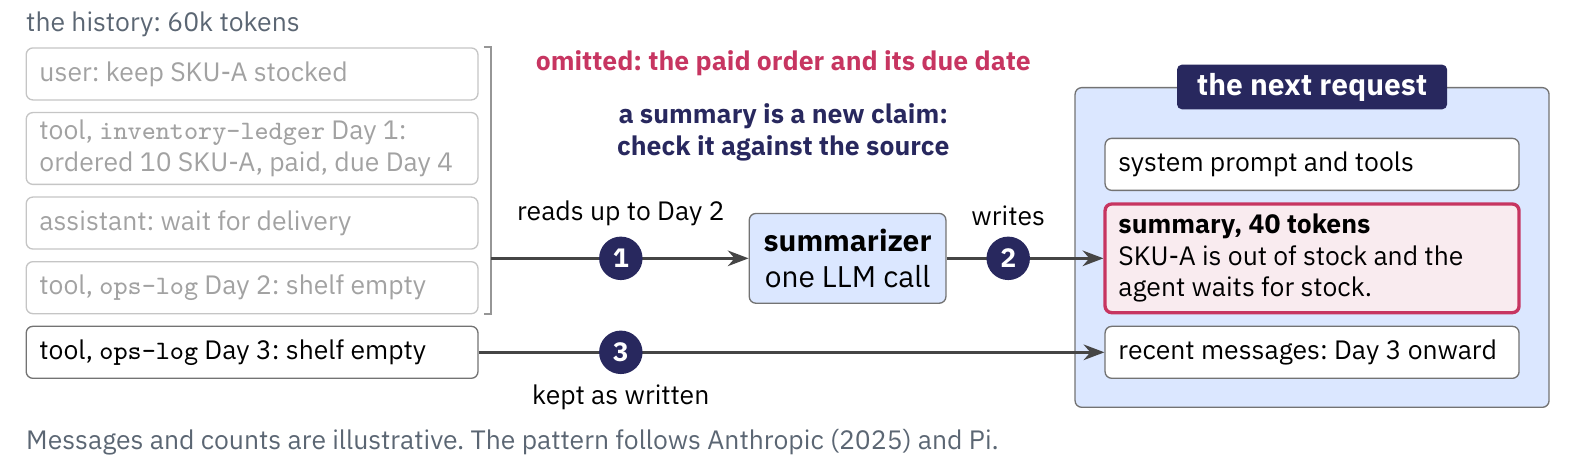
\includegraphics[width=\linewidth]{context/abstractive-4.png}
\caption{Abstractive summary rewrites a span. The figure as it stands after the build's last click.}
\label{fig:abstractive-4}
\end{figure}

\paragraph{The figure, stage by stage.}
\be
\item The next request holds 'system prompt and tools', the summary and 'recent messages: Day 3 onward'. Arrow 3 carries the Day 3 log into it, kept as written.
\item The summary turns magenta, and the magenta line names what it lost: 'omitted: the paid order and its due date'. The navy line names the check: 'a summary is a new claim: check it against the source'.
\ee

\begin{takeaway}A summary restates meaning in new words and needs checking.\end{takeaway}

\subsection{Structured notes hold a running state}
\label{sec:it-7-4d}

\bi
\item \textbf{How:} each step updates a card of goals, open items and decisions.
\item \textbf{Strength:} commitments survive by design.
\item \textbf{Failure:} a fact the schema has no field for is lost.
\ei

Structured notes keep a schema of goals, open items and decisions that each step updates, so a commitment written into the card survives by design. The schema must anticipate what matters: a fact with no field, such as the supplier's warning, has no place to go. Pi uses fixed summary sections and file lists as structured notes (the slide \hyperref[sec:it-7-5a]{``Pi compacts into a structured summary.''}), and Codex can also keep structured memory across sessions when its memories feature is on (the slide ``Codex's local path writes a handoff summary.'').

The card's fields and entries are illustrative. Pi refreshes its fixed sections at each compaction, so a card written at every step is the strategy's idealized form. The failure, a fact with no field, is the course's reasoning, and no source measures how often it happens.

\begin{figure}[htbp]
\centering
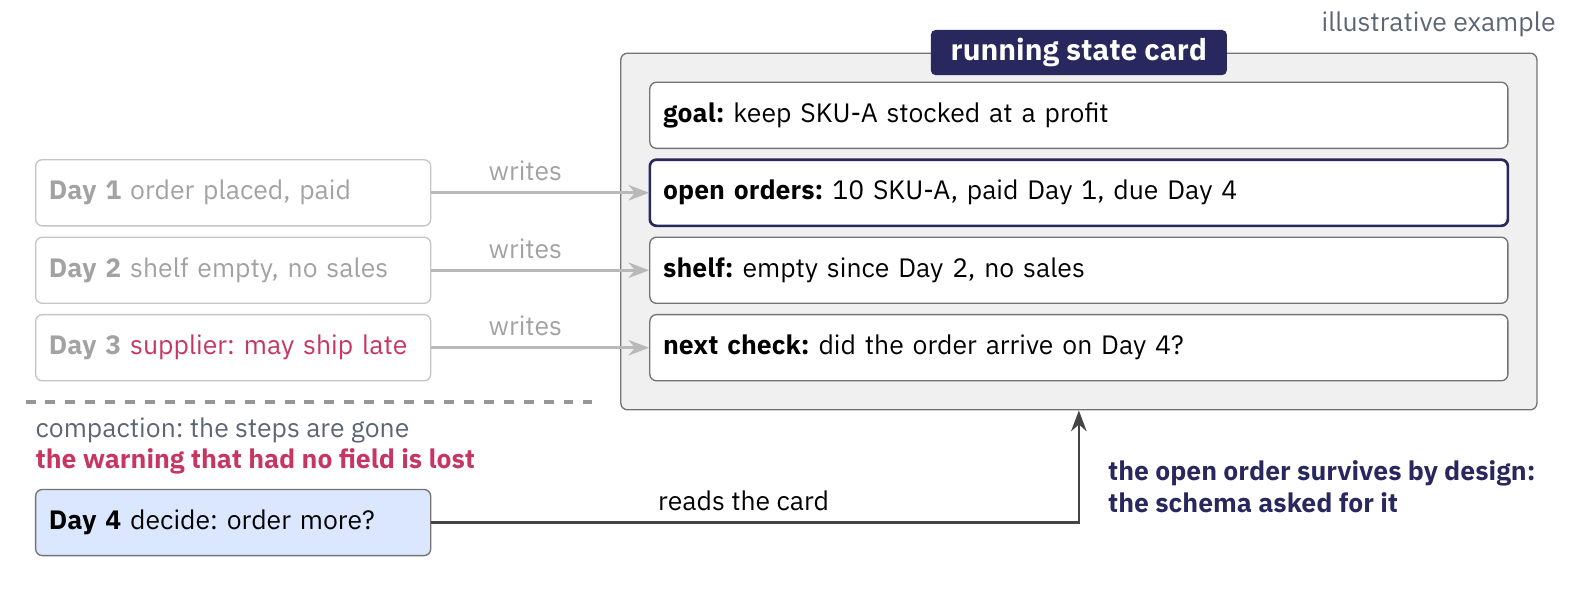
\includegraphics[width=\linewidth]{context/structured-notes-3.png}
\caption{Structured notes hold a running state. The figure as it stands after the build's last click.}
\label{fig:structured-notes-3}
\end{figure}

\paragraph{The figure, stage by stage.}
\be
\item The running state card holds four fields: 'goal: keep SKU-A stocked at a profit', 'open orders: 10 SKU-A, paid Day 1, due Day 4', and two ghosts, 'shelf: none yet' and 'next check: none yet'. The step 'Day 1 order placed, paid' writes the open order into its field.
\item Days 2 and 3 fill the two ghosts: 'Day 2 shelf empty, no sales' writes 'shelf: empty since Day 2, no sales', and 'Day 3 supplier: may ship late' writes 'next check: did the order arrive on Day 4?'. The card has no field for the supplier's warning itself, and the open-orders line stays as Day 1 wrote it.
\item Compaction arrives as a grey dashed rule, 'compaction: the steps are gone', and 'Day 4 decide: order more?' 'reads the card'. In magenta, 'the warning that had no field is lost'. The open-orders field takes a navy outline, and the navy line under the card, where Day 4's arrow enters it, reads 'the open order survives by design: the schema asked for it'.
\ee

\begin{takeaway}A running state card carries commitments across every compaction.\end{takeaway}

\subsection{Sub-agent delegation isolates a context}
\label{sec:it-7-4e}

\bi
\item \textbf{How:} a sub-agent runs a subtask in its own context and returns one result.
\item \textbf{Strength:} the main context stays small.
\item \textbf{Failure:} the result can omit a fact the main agent needs.
\ei

Delegation runs a subtask in its own context and returns one result, so the main context grows by the result alone. The result is lossy: it can omit a fact the main agent needs, such as the supplier's warning, while the sub-agent's reads stay in its own context. Claude Code uses subagents this way (the slide \hyperref[sec:it-7-5b]{``Claude Code summarizes and re-reads files.''}), and the main agent sees the result rather than the subtask's reads.

The token counts and sizes are illustrative, and the short result is a simplification. Claude Code's documentation says that subagents keep large reads outside the main context, and QwenGyre (Wang et al., preprint, 2026, on the slide \hyperref[sec:it-7-5]{``Real harnesses compact, delegate and retry.''}) describes sub-agents with separate contexts. Neither gives sizes or a loss rate, so the loss is a design risk.

\begin{figure}[htbp]
\centering
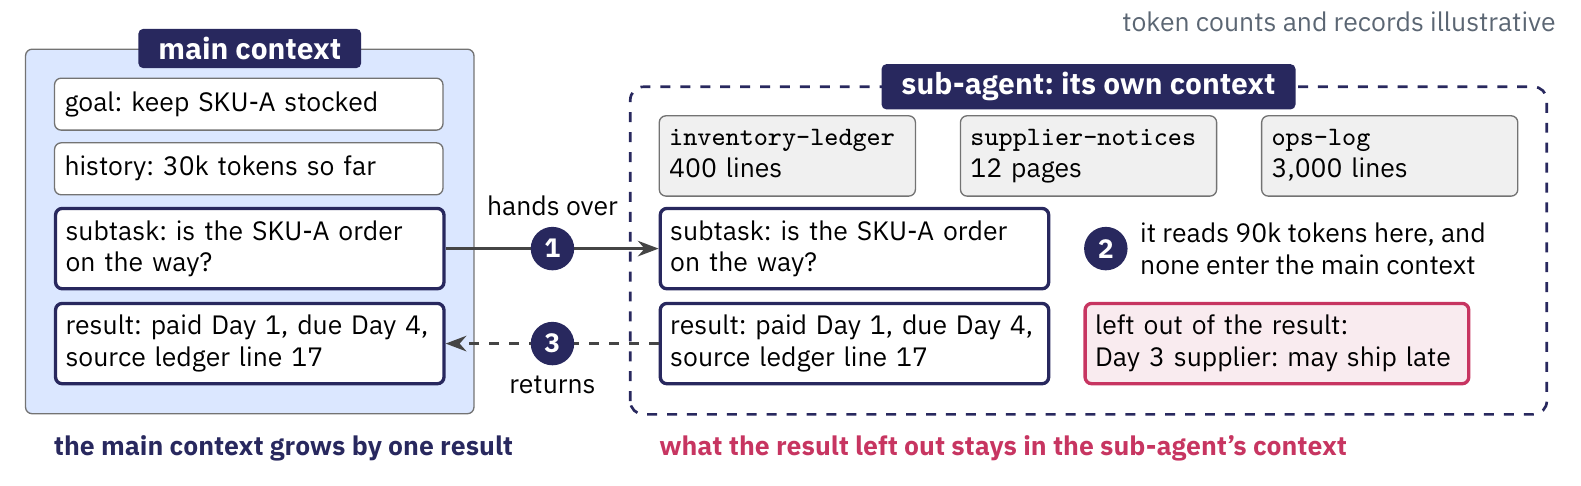
\includegraphics[width=\linewidth]{context/delegation-3.png}
\caption{Sub-agent delegation isolates a context. The figure as it stands after the build's last click.}
\label{fig:delegation-3}
\end{figure}

\paragraph{The figure, stage by stage.}
\be
\item The main context holds 'goal: keep SKU-A stocked', 'history: 30k tokens so far' and the subtask 'is the SKU-A order on the way?'. Event 1 'hands over' the subtask to a sub-agent that works in its own context, and two ghosts marked 'result' show where the answer will go.
\item Three records arrive in the sub-agent's context: inventory-ledger (400 lines), supplier-notices (12 pages) and ops-log (3,000 lines), about 8k, 7k and 75k tokens. Event 2 says 'it reads 90k tokens here, and none enter the main context'.
\item Event 3 'returns' one result, 'result: paid Day 1, due Day 4, source ledger line 17', so 'the main context grows by one result'. The magenta chip 'left out of the result: Day 3 supplier: may ship late' shows that 'what the result left out stays in the sub-agent's context'.
\ee

\begin{takeaway}Delegation moves a subtask's reads out of the main context.\end{takeaway}

\subsection{Retrieval keeps records outside the context}
\label{sec:it-7-4f}

\bi
\item \textbf{How:} records stay in a store outside the context, behind a reference.
\item \textbf{Strength:} it scales past any window.
\item \textbf{Failure:} a query miss or a stale reference.
\ei

Retrieval keeps records in a store outside the context and fetches them by reference when they are needed, so it scales past any window. It fails when a query misses or when a reference has gone stale. Claude Code's re-read of recently touched files after compaction is a bounded form (the slide \hyperref[sec:it-7-5b]{``Claude Code summarizes and re-reads files.''}), and retrieval-augmented generation is the general case. Xu et al. (Retrieval meets Long Context Large Language Models, ICLR 2024) compare the map's two answers directly, a longer window against retrieval: a model with a 4K window and retrieval matched one fine-tuned to a 16K window, and retrieval still helped models with 32K windows.

The store, its line numbers, the cleanup and the counts are illustrative, and the stale reference is a constructed case. The query miss is not drawn. Retrieval scales past any window because the store sits outside it.

\begin{figure}[htbp]
\centering
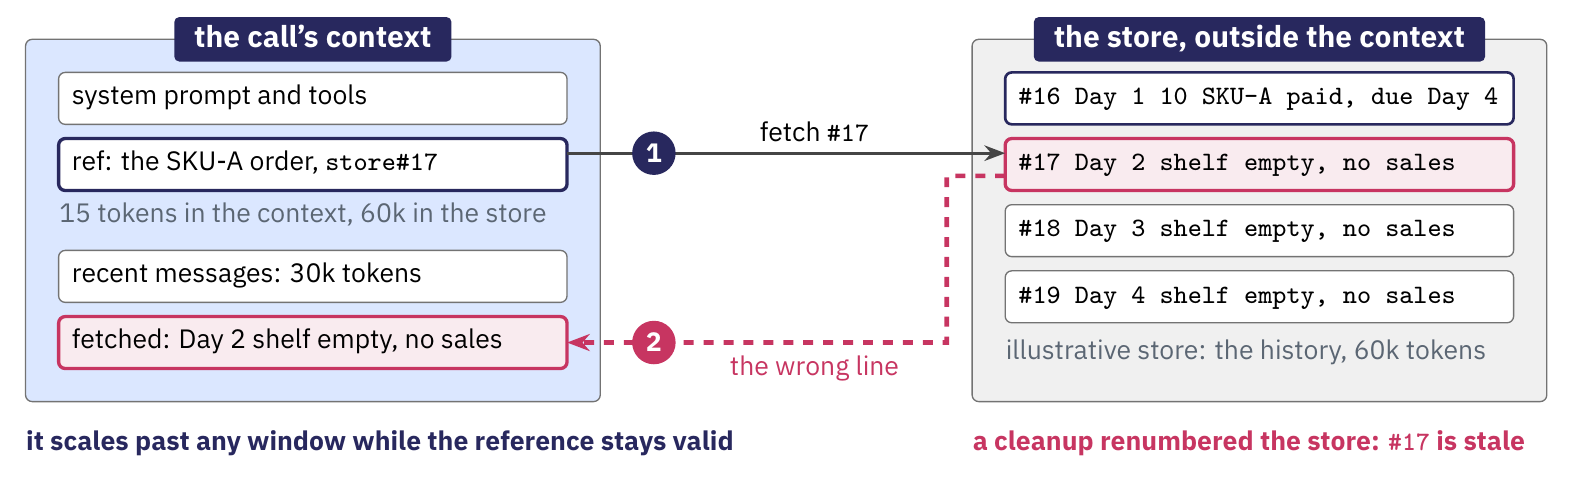
\includegraphics[width=\linewidth]{context/retrieval-3.png}
\caption{Retrieval keeps records outside the context. The figure as it stands after the build's last click.}
\label{fig:retrieval-3}
\end{figure}

\paragraph{The figure, stage by stage.}
\be
\item The call's context keeps a reference where the line would be, ref: the SKU-A order, store\#17, at 15 tokens in the context, 60k in the store. The store, outside the context, holds the history with the paid order at \#17, and the ghost marks where the fetched line will go.
\item Fetch \#17 reaches row \#17, and the line comes back word for word as fetched: Day 1 10 SKU-A paid, due Day 4. The paid order enters the context when the decision needs it.
\item A cleanup renumbered the store: \#17 is stale, so the same fetch returns the wrong line, Day 2 shelf empty, no sales, while the paid order sits at \#16. The navy line states the condition: it scales past any window while the reference stays valid.
\ee

\begin{takeaway}Retrieval trades in-context text for a fetch when it is needed.\end{takeaway}

\subsection{Compaction strategies compared}
\label{sec:it-7-4g}

\textbf{This table recaps the strategies of the previous slides.}

This table recaps the six strategy slides, one row per click. Each strategy buys room by giving up a different kind of recall: recency the oldest commitment, extraction the words it drops, a summary what it omits, structured notes what the schema has no field for, delegation what the result leaves out, and retrieval what a query misses.

The strategies use the four ways of the slide \hyperref[sec:it-7-1]{``Context: retain, retrieve, extract, rewrite''}. Recency retains the newest turns as written, extractive selection extracts, an abstractive summary rewrites, and structured notes rewrite the run's state into fields. Retrieval on demand is the retrieve way, and delegation moves a subtask's reads into a context of its own.

KV-cache eviction works at a different layer, the models lane of the map. StreamingLLM (Xiao et al., Efficient Streaming Language Models with Attention Sinks, ICLR 2024) and H2O (Zhang et al., H2O: Heavy-Hitter Oracle for Efficient Generative Inference of Large Language Models, NeurIPS 2023) reduce the cached activations inside the model, and the strategies in this table change the input text.

\begin{center}\footnotesize
\begin{tabularx}{\linewidth}{L{0.22\linewidth}XXX}
\toprule
\textbf{Strategy} & \textbf{How it works} & \textbf{Strength} & \textbf{Main failure} \\
\midrule
Recency or truncation & Keep the last turns, drop older ones & No extra compute & Drops an old but open commitment \\
Extractive selection & Keep the informative tokens (LLMLingua-2) & Cheap, model-agnostic & Lexical choice can shed meaning \\
Abstractive summary & Rewrite a span into a shorter account & Preserves meaning flexibly & Omission and unsupported claims \\
Structured notes & Keep a running state of goals and open items & Commitments persist by design & The schema must anticipate needs \\
Sub-agent delegation & Run a subtask in an isolated context & Keeps the main context small & The result can omit a needed fact \\
Retrieve on demand & Store records outside, fetch by reference & Scales past any window & A query miss or a stale reference \\
\bottomrule
\end{tabularx}
\end{center}

\begin{takeaway}Each strategy buys room by giving up a different kind of recall.\end{takeaway}

\subsection{Real harnesses compact, delegate and retry}
\label{sec:it-7-5}

\bi
\item \textbf{Compaction:} a full window becomes a summary, and the run continues from it.
\item \textbf{Delegation:} a sub-agent works in its own context and returns one result.
\item \textbf{Retries:} a failed path runs again, so one task becomes a graph of paths.
\item \textbf{The scale:} hours, hundreds of interactions, nearly 1M tokens (a 2026 preprint).
\ei

Wang et al., QwenGyre: An Elastic Reinforcement Learning Framework for Training xLong-Horizon Agents, arXiv:2609.33848, version 2, October 20, 2026 (version 1, September 27), Alibaba, a preprint. Its contribution is reinforcement-learning training infrastructure, and we cite its account of real harnesses. When the window fills, the harness compacts the saturated history into a summary branch that replaces the history before it, and the run continues from the summary. Sub-agents hold separate contexts and return their result to the main agent. A failed branch is retried, so one task becomes a graph of context paths.

Continuously, because the harness compacts again each time a window fills. In layers, because sub-agents compact too: in the paper's traced run, the main agent and a sub-agent each compact their own context (appendix C.2).

The scale is the paper's xLong profile: a single run can span hours, hundreds of model--environment interactions and nearly 1M input and output tokens across its model calls. That count repeats the context of every request, so it can exceed the context limit of a single request (section 2.1). The profile describes the xLong executions the paper focuses on (section 2.1). Of its three workloads, NL2RepoBench, DeepSWE and TerminalBench, the paper calls NL2RepoBench the xLong setting, and all three ran through Claude Code 2.1.220 (section 6.1). Later systems may differ. The report is very recent and has almost no citations yet.

The eleven steps and their wiring are illustrative: the compaction after step 5, the sub-agent that leaves step 8 and returns one result to step 9, and the failed path at step 10 with its retry into step 11. The paper supplies the three mechanisms, compacted saturated histories, sub-agents with isolated contexts and retried failed paths, and the scale of its own runs.

\begin{figure}[htbp]
\centering
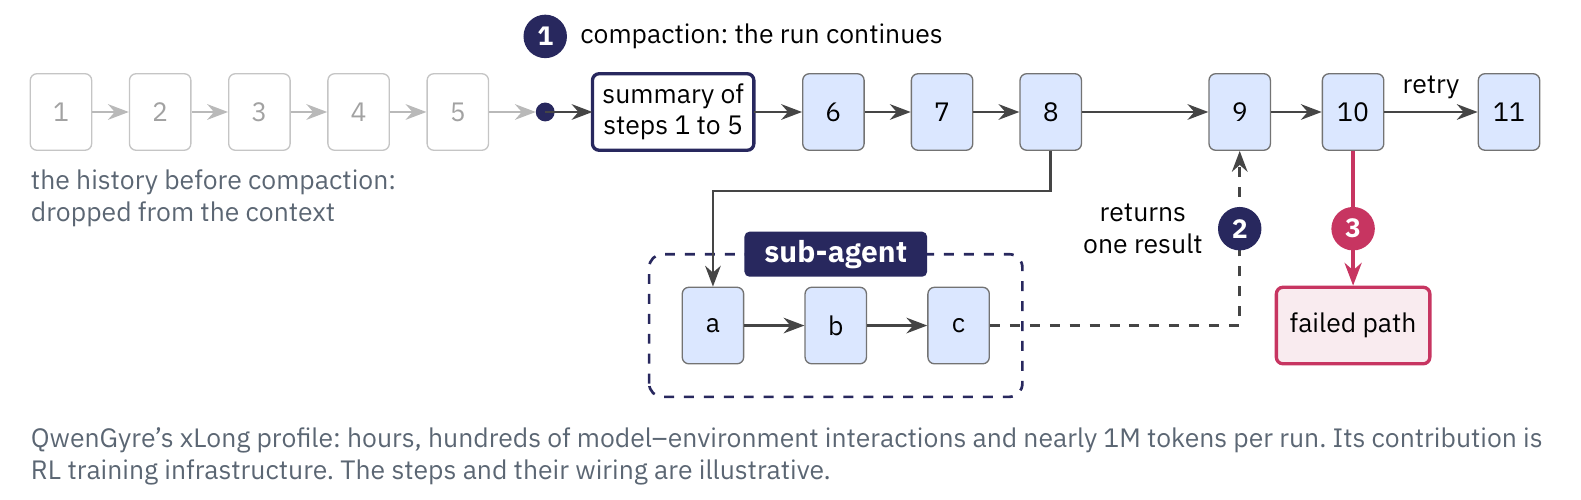
\includegraphics[width=\linewidth]{context/harness-branches-3.png}
\caption{Real harnesses compact, delegate and retry. The figure as it stands after the build's last click.}
\label{fig:harness-branches-3}
\end{figure}

\paragraph{The figure, stage by stage.}
\be
\item Compaction: after step 5 the harness writes the summary of steps 1 to 5, and the run continues from it through step 11. Steps 1 to 5 are the history before compaction, dropped from the context, so no later step sees them.
\item Sub-agent: step 8 hands a subtask to a sub-agent, which runs steps a, b and c in its own context. The sub-agent returns one result to step 9, so the main run never holds steps a, b and c.
\item Failed path: step 10 starts a path that fails, and the harness retries, so the arrow from step 10 to step 11 is the retry. The run is now a graph of context paths, and the note gives QwenGyre's xLong profile: hours, hundreds of model--environment interactions and nearly 1M tokens per run.
\ee

\begin{takeaway}At extreme-long horizons, compaction runs continuously and in layers.\end{takeaway}

\subsection{Pi compacts into a structured summary}
\label{sec:it-7-5a}

\bi
\item \textbf{Summary:} an LLM rewrites the older messages into one summary.
\item \textbf{Recency:} the most recent messages stay, about 20k tokens.
\item \textbf{Structured notes:} fixed sections, from Goal to Critical Context, and file lists.
\ei

Pi 1.2.0's docs/compaction.md describes its compaction. Automatic compaction starts when the tokens in context exceed the context window minus a reserve, 16384 tokens by default, and the user can also enter /compact. Pi keeps the most recent messages, about 20k estimated tokens (keepRecentTokens, a target rather than a cap), summarizes the older ones with an LLM, and rebuilds the context from the system prompt, the summary and the kept messages. The summary has fixed sections: Goal, Constraints \& Preferences, Progress (done, in progress, blocked), Key Decisions, Next Steps and Critical Context. Cumulative lists of the files read and modified follow, and a later compaction includes the previous summary. When the cut falls inside one prompt's span of messages, Pi also summarizes the start of that span under its own headings (Original Request, Progress So Far, Context Needed to Continue) and appends it as a Turn Context section. With earlier messages to summarize as well, that takes a second call.

Pi combines three strategies of the earlier slides: an abstractive summary, recency, and structured notes in its sections and file lists. The defaults are current values that can change.

Pi's documentation describes behaviour and measures nothing.

\begin{figure}[htbp]
\centering
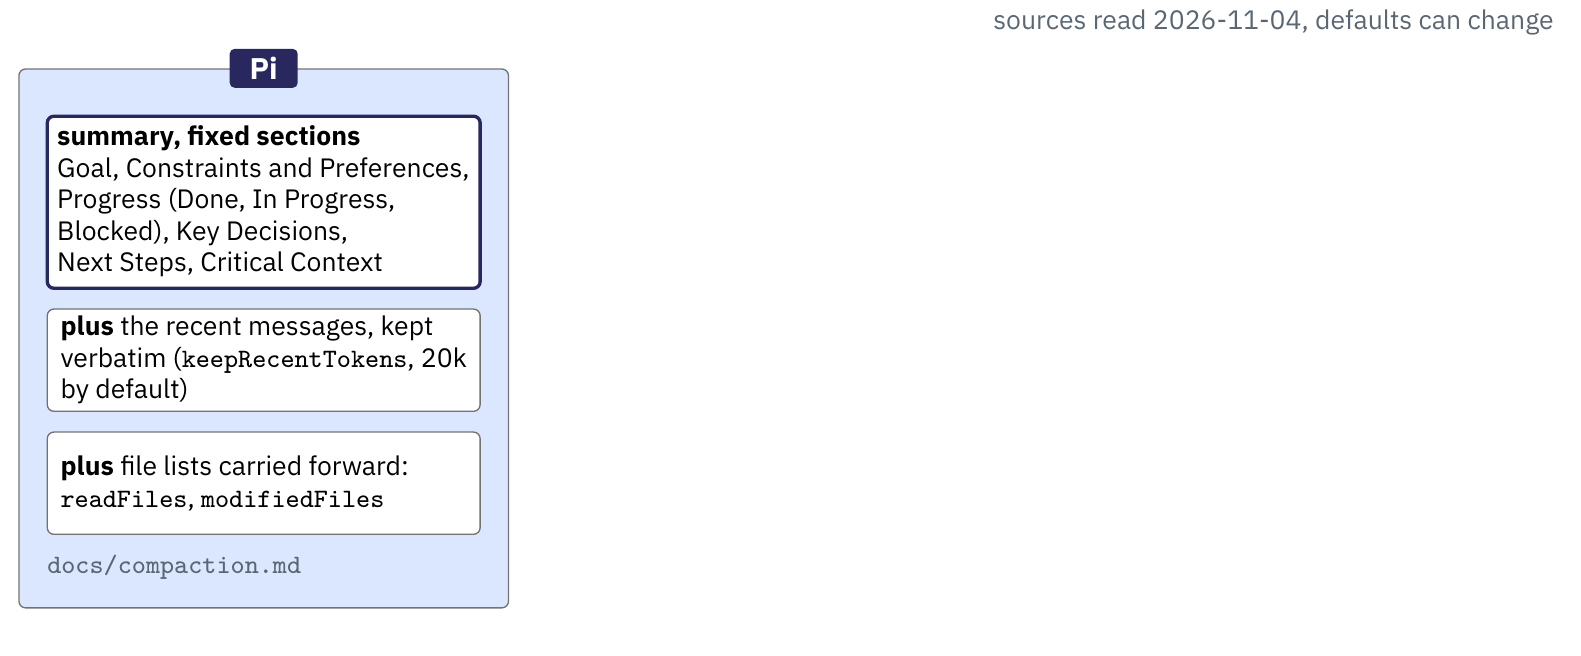
\includegraphics[width=\linewidth]{context/harness-formats-1.png}
\caption{Pi compacts into a structured summary. The figure as it stands after the build's last click.}
\label{fig:harness-formats-1}
\end{figure}

\paragraph{The figure, stage by stage.}
\be
\item The Pi column comes first: a 'summary, fixed sections', from 'Goal' to 'Critical Context', replaces the older messages. Pi also keeps 'the recent messages, kept verbatim (keepRecentTokens, 20k by default)', and its 'file lists carried forward: readFiles, modifiedFiles'.
\ee

\begin{takeaway}Pi pairs a summary with the most recent messages and structured notes.\end{takeaway}

\subsection{Claude Code summarizes and re-reads files}
\label{sec:it-7-5b}

\bi
\item \textbf{Summary:} the conversation becomes a structured summary.
\item \textbf{Retrieval:} it re-reads up to five recently touched files.
\item \textbf{Delegation:} its subagents keep large reads in separate contexts.
\ei

Claude Code's documentation describes its compaction (Explore the context window, \url{https://code.claude.com/docs/en/context-window}, and How Claude Code works, \url{https://code.claude.com/docs/en/how-claude-code-works}, read November 4, 2026). Automatic compaction runs as the window fills, and the user can also enter /compact with a focus. Claude Code replaces the conversation with a structured summary, then reads up to five recently touched files again. A file over 5000 tokens returns as a path reference. SessionStart hooks with the compact source add their output again, the text of skills returns within a limit for each skill, and subagents keep large reads in separate contexts.

Claude Code combines an abstractive summary with retrieval of recent files and with delegation. The thresholds are current values that can change.

Claude Code also compacts at the threshold that /autocompact sets. Its documentation describes behaviour and measures nothing.

\begin{figure}[htbp]
\centering
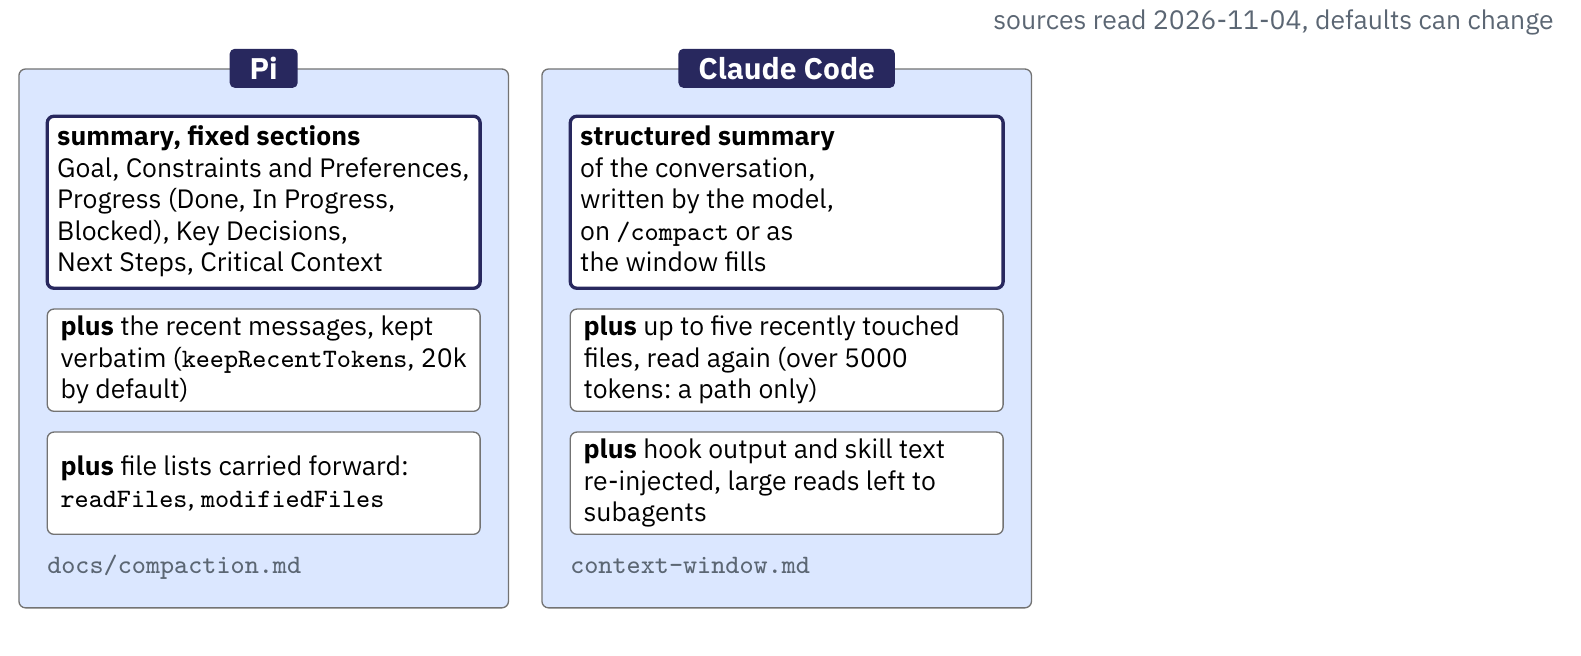
\includegraphics[width=\linewidth]{context/harness-formats-2.png}
\caption{Claude Code summarizes and re-reads files. The figure as it stands after the build's last click.}
\label{fig:harness-formats-2}
\end{figure}

\paragraph{The figure, stage by stage.}
\be
\item The Pi column comes first: a 'summary, fixed sections', from 'Goal' to 'Critical Context', replaces the older messages. Pi also keeps 'the recent messages, kept verbatim (keepRecentTokens, 20k by default)', and its 'file lists carried forward: readFiles, modifiedFiles'.
\item The Claude Code column adds a 'structured summary' of the conversation, 'written by the model, on /compact or as the window fills'. Under it Claude Code reads 'up to five recently touched files' again (a file 'over 5000 tokens' comes back as 'a path only') and re-injects 'hook output and skill text', while 'large reads' are 'left to subagents'.
\ee

\begin{takeaway}Claude Code pairs a summary with a recent-file re-read.\end{takeaway}

\subsection{Codex's local path writes a handoff summary}
\label{sec:it-7-5c}

\bi
\item \textbf{Summary:} a context-checkpoint handoff summary for the next model.
\item \textbf{Retain:} it keeps the user's latest messages beside the summary.
\item \textbf{Structured notes:} an opt-in memories pipeline across sessions.
\ei

The compaction prompt is in the openai/codex repository at commit de6e72a, read November 4, 2026 (codex-rs/prompts/templates/compact/prompt.md and summary\_prefix.md). It calls the step context checkpoint compaction and asks for a handoff summary for another model that will resume the task: progress and key decisions, important context and user preferences, next steps, and critical data or references. Codex rebuilds the history from that summary and the user's most recent messages, up to 20,000 tokens (core/src/compact.rs). It also tells the next model that it still has access to the state of the tools the previous model used, which persists outside the context.

This is the local path. With the default OpenAI provider, Codex uses the remote compaction of the Responses API instead (model-provider/src/capabilities.rs), and the repository shows the summary format only for the local path, which other providers use. Codex compacts automatically when token use reaches its auto-compact limit (model\_auto\_compact\_token\_limit, or the model's default), and the user can also enter /compact. It keeps resume metadata for its sessions, and a memories pipeline, off by default, extracts structured memory across sessions when it is enabled.

Codex combines an abstractive summary with retained user messages and, when enabled, structured notes across sessions.

The memories pipeline runs beside compaction rather than inside it. The repository describes behaviour and measures nothing.

\begin{figure}[htbp]
\centering
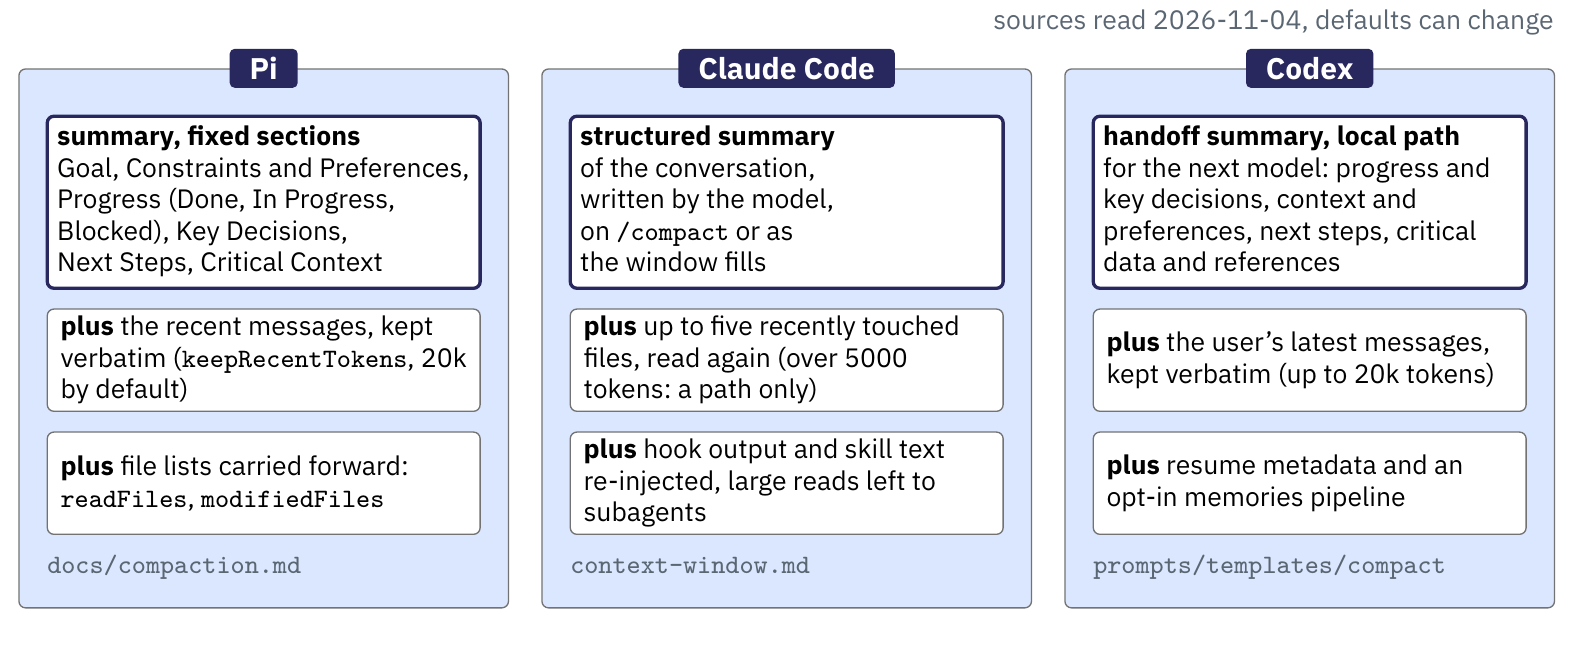
\includegraphics[width=\linewidth]{context/harness-formats-3.png}
\caption{Codex's local path writes a handoff summary. The figure as it stands after the build's last click.}
\label{fig:harness-formats-3}
\end{figure}

\paragraph{The figure, stage by stage.}
\be
\item The Claude Code column adds a 'structured summary' of the conversation, 'written by the model, on /compact or as the window fills'. Under it Claude Code reads 'up to five recently touched files' again (a file 'over 5000 tokens' comes back as 'a path only') and re-injects 'hook output and skill text', while 'large reads' are 'left to subagents'.
\item The Codex column adds a 'handoff summary, local path': when Codex compacts locally, the model writes a summary 'for the next model: progress and key decisions, context and preferences, next steps, critical data and references'. Beside the summary Codex keeps 'the user's latest messages, kept verbatim (up to 20k tokens)', and the third box adds 'resume metadata and an opt-in memories pipeline'.
\ee

\begin{takeaway}Codex pairs a handoff summary with the user's latest messages.\end{takeaway}

\subsection{The harness formats share an abstractive core}
\label{sec:it-7-5d}

The last stage frames the three summaries in navy. All three harnesses build compaction on an abstractive, structured summary, and each adds a second strategy of its own: Pi keeps the most recent messages, Claude Code re-reads recent files, and Codex keeps the user's latest messages. Codex's summary is that of its local path. With the default OpenAI provider, Codex compacts on the server, which returns an encrypted item whose format the repository does not show. The sources are those of the three previous slides.

\begin{figure}[htbp]
\centering
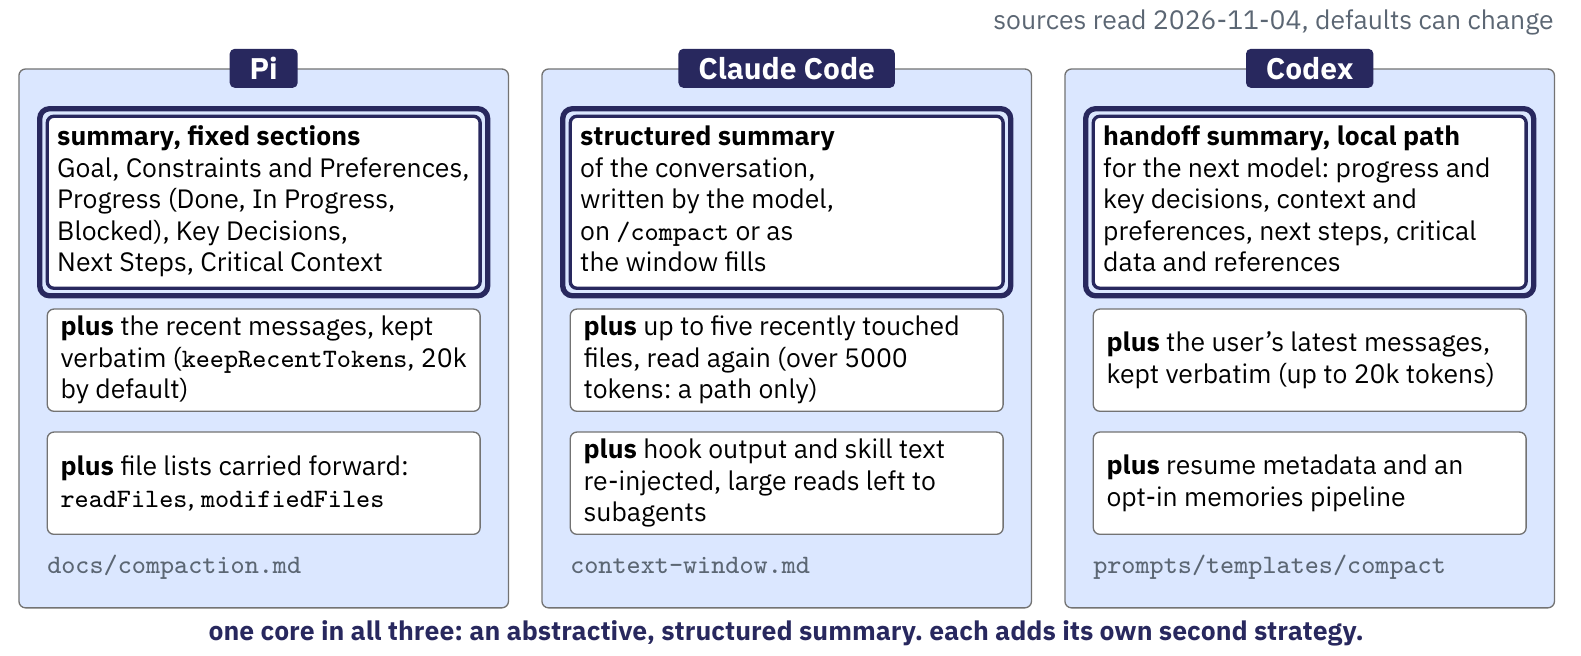
\includegraphics[width=\linewidth]{context/harness-formats-4.png}
\caption{The harness formats share an abstractive core. The figure as it stands after the build's last click.}
\label{fig:harness-formats-4}
\end{figure}

\paragraph{The figure, stage by stage.}
\be
\item The navy frames mark the core all three share, and the caption reads 'one core in all three: an abstractive, structured summary. each adds its own second strategy.' Pi keeps the recent messages, Claude Code reads recent files again, and Codex keeps the user's latest messages.
\ee

\begin{takeaway}Pi, Claude Code and Codex build compaction on an abstractive summary.\end{takeaway}

\subsection{Harness formats compared}
\label{sec:it-7-5e}

\textbf{This table groups the harnesses by the earlier strategies.}

This table recaps the three harness slides, one row per click, in the names of the strategy slides. Pi keeps the most recent messages, Claude Code re-reads recent files and delegates to subagents, and Codex keeps the user's latest messages. Codex's summary format belongs to its local path. With the default OpenAI provider, Codex compacts on the server. The sources are those of the three harness slides, collected in drafts/section-specs/part-02-harness-compaction.md of the lecture folder.

\begin{center}\footnotesize
\begin{tabularx}{\linewidth}{L{0.22\linewidth}XXX}
\toprule
\textbf{Harness} & \textbf{Core} & \textbf{Second strategy} & \textbf{Further strategies} \\
\midrule
Pi & Abstractive structured summary & Recency: recent messages & Structured notes: file lists \\
Claude Code & Abstractive structured summary & Retrieval: recent files & Delegation: subagents \\
Codex & Abstractive handoff summary (local path) & Retain: recent user messages & Structured notes: opt-in memories \\
\bottomrule
\end{tabularx}
\end{center}

\begin{takeaway}Each harness pairs an abstractive summary with other compaction strategies.\end{takeaway}

\subsection{LangGraph can compact one call or the thread}
\label{sec:it-7-6}

\bi
\item \textbf{One call:} \texttt{trim\_messages} or context editing shortens the model's input.
\item \textbf{The thread:} \texttt{SummarizationMiddleware} rewrites the old messages.
\item \textbf{A file:} Deep Agents moves a large tool result out and keeps a preview.
\ei

The coding harnesses compact in their own ways. LangGraph, the framework the course builds agents with, leaves the choice to the developer. It saves an agent's state per thread: the checkpointer writes a checkpoint after every step, so the thread is the agent's short-term memory, and a Store keeps long-term memory across threads. LangChain v1's create\_agent compiles to a LangGraph graph, and its middleware supplies the packaged strategies. We read langchain 1.4.9, langgraph 1.2.20 and deepagents 0.7.32, with their documentation, on November 5, 2026.

For each strategy we ask where its change lands. trim\_messages, from langchain-core, returns a shorter list for one call, and the thread keeps every message. ContextEditingMiddleware with ClearToolUsesEdit also changes one call: it replaces older tool results with ``[cleared]'' in what the model receives, and its source says that it mirrors Anthropic's context editing. SummarizationMiddleware changes the thread: before the model call it writes RemoveMessage(REMOVE\_ALL\_MESSAGES), a summary and the recent messages into the state, and it never separates a tool call from its result. The thread's earlier checkpoints still hold the old messages. Deep Agents, LangChain's agent harness built on LangGraph, moves a tool result of more than 20,000 tokens into a file under /large\_tool\_results/ and keeps a preview of its first and last lines, and its own summarizer keeps the cut history in a file. A developer can also write a @before\_model hook, which changes the thread, or a @wrap\_model\_call hook, which changes one call. The pre\_model\_hook of create\_react\_agent is deprecated.

These map onto the strategies of the earlier slides. Trimming keeps the most recent turns, clearing old tool results masks observations, the summary is abstractive, the file is retrieval by reference, and Deep Agents' subagents delegate.

The numbers in the figure come from a demonstration on the vending run, which the next slide quotes. Its 13 messages hold the Day 1 order in m04 and m05 and the Day 4 request in m13. trim\_messages with max\_tokens=300 returns m10 to m13, so that call never sees the order. SummarizationMiddleware removes m01 to m07, so only the summary carries the order. ClearToolUsesEdit replaces the order confirmation, m05, with ``[cleared]'', while the agent's own message m06 still states the order.

The vending history is scripted, and the message labels, the counts and the tokens come from the capture of the demonstration. The figure leaves out context editing, the Store and subagents, which the notes name. Where the documentation and the code disagree, the research note drafts/section-specs/part-02-langgraph-compaction.md records both.

\begin{figure}[htbp]
\centering
\includegraphics[width=\linewidth]{context/langgraph-compaction-4.png}
\caption{LangGraph can compact one call or the thread. The figure as it stands after the build's last click.}
\label{fig:langgraph-compaction-4}
\end{figure}

\paragraph{The figure, stage by stage.}
\be
\item The thread: LangGraph's checkpointer saves the vending run's thread vm-1, ``13 messages, about 730 tokens'', with ``a checkpoint after every step''. The Day 1 order is m04 and m05, and m13 is the Day 4 request. The grey note names the demonstration, demo.py, run with LangChain 1.4.9.
\item One call: ``trim\_messages: the model receives m10 to m13'', while ``the thread still holds all 13 messages'', so the Day 1 order is ``not in this call'' and comes back on the next one.
\item The thread: ``SummarizationMiddleware: a summary replaces m01 to m07'', and ``the model receives the summary and m08 to m13'', so for ``the Day 1 order'', ``the model sees it only in the summary''. The step-0 checkpoint still holds all 13 messages, which the next slide's capture shows. The one-call box settles to a grey outline.
\item A file: ``Deep Agents: a large tool result moves to a file'', and ``a preview stays, and read\_file reads the rest''. The Day 1 order is ``a short result, so it stays''.
\ee

\begin{takeaway}Each LangGraph compaction changes one call, the thread or a file.\end{takeaway}

\subsection{SummarizationMiddleware rewrites the thread}
\label{sec:it-7-7}

\bi
\item \textbf{The trigger:} past 600 tokens, a summary replaces all but six messages.
\item \textbf{The capture:} the thread loses m01 to m07, and the summary keeps the order.
\ei

The window quotes slides/demos/langgraph/demo.py, lines 161 to 171, and the output quotes four lines of its capture, demo.out.txt, of November 5, 2026, with Python 3.13.15, langchain 1.4.9, langgraph 1.2.20, langchain-core 1.7.6 and langgraph-checkpoint 4.3.1. Both models in the demonstration are fakes (GenericFakeChatModel), so the history, the summary and the agent's reply are scripted. The libraries count the tokens, decide when to summarize, choose the cut, rewrite the state and save the checkpoints.

create\_agent takes the middleware list, and SummarizationMiddleware runs as the node SummarizationMiddleware.before\_model before each model call. trigger=(``tokens'', 600) fires once the thread's messages reach 600 tokens, counted approximately, and keep=(``messages'', 6) keeps the six newest messages as written. A trigger can also count messages or a fraction of the model's input limit, and without one the middleware never runs. By default it keeps 20 messages. The checkpointer, InMemorySaver here, saves the thread at every step.

The capture shows the rewrite. At step 0 the thread holds 13 messages, about 730 tokens. The node writes RemoveMessage(id=''\_\_remove\_all\_\_''), a summary and m08 to m13, so at step 1 the model receives 7 messages. The removed messages, m01 to m07, include the Day 1 order (m04 and m05). The scripted summary keeps the order, its due date and its source: ``Order 17: 10 SKU-A, paid 30.00, due Day 4 (source: inventory-ledger, Day 1)''. A real summarizer writes its own words, and whether they keep the order is the question of the slide \hyperref[sec:it-9-3]{``Each summary leads to a different decision.''} The earlier checkpoints still hold all 13 messages, so the thread's history can recover them, but the agent no longer sees them.

The 600-token trigger suits a short demonstration. Real triggers sit near the model's window: Deep Agents, for example, summarizes at 85 percent of the model's input limit.

\paragraph{demo.py: summarize past 600 tokens, keep the six newest messages}
\begin{footnotesize}
\begin{verbatim}
agent = create_agent(
    model=agent_model,
    middleware=[
        SummarizationMiddleware(
            model=summarizer,          # writes the summary
            trigger=("tokens", 600),   # past 600 tokens in the thread
            keep=("messages", 6),      # the 6 newest stay as written
        ),
    ],
    checkpointer=InMemorySaver(),
)
\end{verbatim}
\end{footnotesize}

\paragraph{output: the checkpoints of thread vm-1, captured November 5, 2026}
\begin{footnotesize}
\begin{verbatim}
step 0  next: SummarizationMiddleware.before_model  13 messages, ~730 tokens
step 1  next: model                                  7 messages, ~502 tokens
the node wrote RemoveMessage(id='__remove_all__'), a summary, m08 to m13
removed from the thread: m01 to m07, the Day 1 order (m04, m05) among them
\end{verbatim}
\end{footnotesize}

\begin{takeaway}A summary that rewrites the thread must carry every open commitment.\end{takeaway}

\subsection*{Key points}
\bi
\item A context policy determines what to keep, fetch, shorten or rewrite.
\item A compressed input is judged by the task it must support.
\item A generated summary becomes another representation that needs checking.
\item Newer compaction is measured, and often trained, on the agent's own tasks.
\item Recency adds no cost, and an open commitment leaves with its old turns.
\item Extraction shortens the text and keeps the original words.
\item A summary restates meaning in new words and needs checking.
\item A running state card carries commitments across every compaction.
\item Delegation moves a subtask's reads out of the main context.
\item Retrieval trades in-context text for a fetch when it is needed.
\item Each strategy buys room by giving up a different kind of recall.
\item At extreme-long horizons, compaction runs continuously and in layers.
\item Pi pairs a summary with the most recent messages and structured notes.
\item Claude Code pairs a summary with a recent-file re-read.
\item Codex pairs a handoff summary with the user's latest messages.
\item Pi, Claude Code and Codex build compaction on an abstractive summary.
\item Each harness pairs an abstractive summary with other compaction strategies.
\item Each LangGraph compaction changes one call, the thread or a file.
\item A summary that rewrites the thread must carry every open commitment.
\ei
